\subsubsection{ΠΕΡΙΠΤΩΣΗ ΧΡΗΣΗΣ 3: ADMIN}
	
\subsubsubsection{Χρήστες (ρόλοι) που εμπλέκονται}
Στη συγκεκριμένη περίπτωση χρήσης εμπλέκεται ο "Διαχειριστής", ο οποίος αλληλεπιδρά με το ειδικό dashboard που εμφανίζεται λόγω της ιδιότητάς του.

\subsubsubsection{Προϋποθέσεις Εκτέλεσης}
Οι συνθήκες οι οποίες πρέπει να πληρούνται είναι:
\begin{enumerate}
	\item σύνδεση στο διαδίκτυο
	\item η βάση δεδομένων του backend είναι online
	\item η διαδικτυακή διεπαφή λειτουργεί
	\item η διεπαφή με το API του MapBox είναι ενεργή
	\item ο χρήστης που προσπαθεί να κάνει login πρέπει να έχει credentials διαχειριστή
\end{enumerate}

\subsubsubsection{Περιβάλλον Εκτέλεσης}
Το περιβάλλον στο οποίο εκτελείται η περίπτωση χρήσης είναι η διαδικτυακή διεπαφή χρήστη, το οποίο μετατρέπεται σε dashboard μετά το επιτυχημένο login, είτε από κάποιο φυλλομετρητή, είτε από κάποιο smartphone.

\subsubsubsection{Δεδομένα Εισόδου}
Τα δεδομένα εισόδου είναι:
\begin{enumerate}
	\item username
	\item password
\end{enumerate}
Η εγκυρότητα των άνω έγκειται στο γεγονός ότι τα credentials αντιστοιχούν σε ένα χρήστη που έχει ρόλο διαχειριστή.
Τα δεδομένα εξόδου είναι:
\begin{enumerate}
	\item επιτυχής διαγραφή χρήστη
	\item επιτυχής αναβάθμιση χρήστη σε διαχειριστή
	\item επιτυχής διαγραφή καταστήματος
\end{enumerate}
Η εγκυρότητα των άνω έγκειται στο γεγονός ότι ο διαχειριστής χρησιμοποιεί σωστά τις λειτουργικότητες που παρέχει η διαδικτυακή διεπαφή, ενώ ταυτόχρονα τα δεδομένα που εμφανίζονται από αυτή είναι συνεπή με τη βάση δεδομένων μας.

\subsubsubsection{Παράμετροι}
Δεν υπάρχουν παράμετροι

\subsubsubsection{Αλληλουχία Ενεργειών - Επιθυμητή Συμπεριφορά}
Τα βήματα που απαιτούνται για την περίπτωση χρήσης είναι:
\begin{enumerate}
	\item εισαγωγή username και password για σύνδεση διαχειριστή
	\item επιβεβαίωση ρόλου διαχειριστή
	\item φόρτωση δεδομένων εμφάνισης
	\item εμφάνιση dashboard
	\item επιτέλευση λειτουργίας
	\begin{enumerate}
		\item Διαγραφή Χρήστη
		\begin{itemize}
			\item κλικ "Χρήστες"
			\item εμφάνιση χρηστών σε λίστα
			\item κλικ "Διαγραφή" σε κάποιο χρήστη
		\end{itemize}
		\item Διαγραφή Καταστήματος
		\begin{itemize}
			\item κλικ "Καταστήματα"
			\item εμφάνιση καταστημάτων σε λίστα
			\item κλικ "Διαγραφή" σε κάποιο κατάστημα
		\end{itemize}
		\item Προαγωγή Χρήστη σε Admin
		\begin{itemize}
			\item κλικ "Χρήστες"
			\item εμφάνιση χρηστών σε λίστα
			\item κλικ "Προαγωγή" σε κάποιο χρήστη
		\end{itemize}
	\end{enumerate}
\end{enumerate}
Ένα γενικό Activity Diagram για τις ενέργειες του διαχειριστή είναι το \ref{fig:Admin_Activity}.
Το Sequence Diagram για το login as administrator και την εμφάνιση του dashboard είναι το \ref{fig:Admin_Login}.
(Οι υπόλοιπες ενέργειες αναφέρονται στα \textbf{Δεδομένα εξόδου})

\subsubsubsection{Δεδομένα εξόδου}
Εξετάζονται οι ακόλουθες περιπτώσεις για τον "Διαχειριστή":
\begin{itemize}
	\item Διαγραφή χρήστη, βλ. \ref{fig:Admin_Delete_User}
	\item Διαγραφή καταστήματος, βλ. \ref{fig:Admin_Delete_Store}
	\item Ενημέρωση χρήστη. βλ, \ref{fig:Admin_Update_User}
\end{itemize}


\begin{figure}[H]
    \centering
    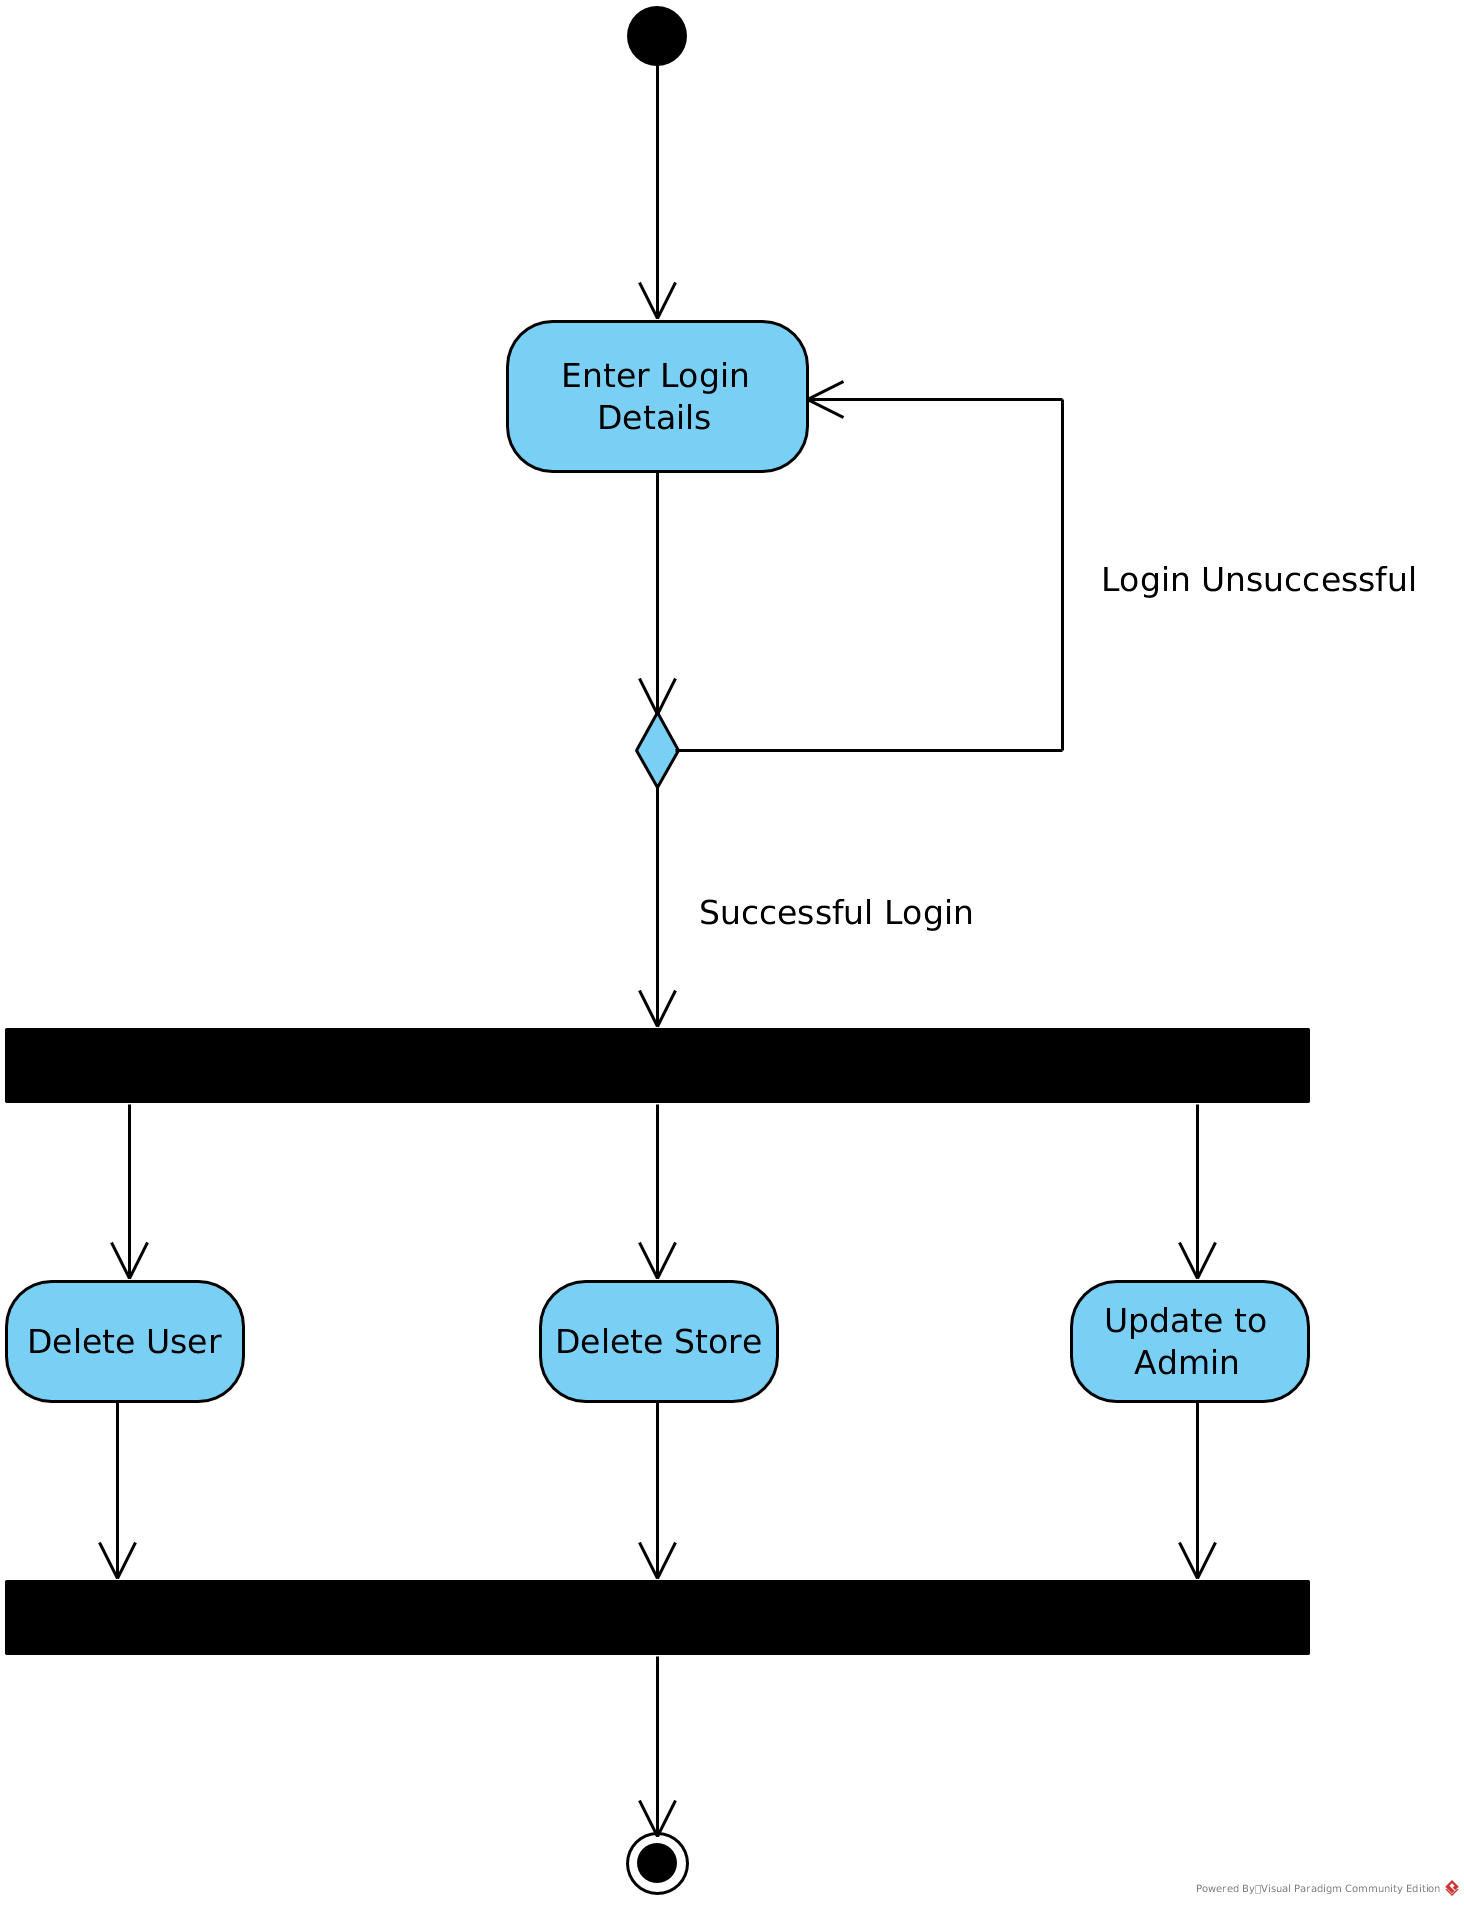
\includegraphics[]{media/Activity/Admin.png}
	\caption{Admin: Activity Diagram}
	\label{fig:Admin_Activity}
\end{figure}



\begin{figure}[H]
    \centering
    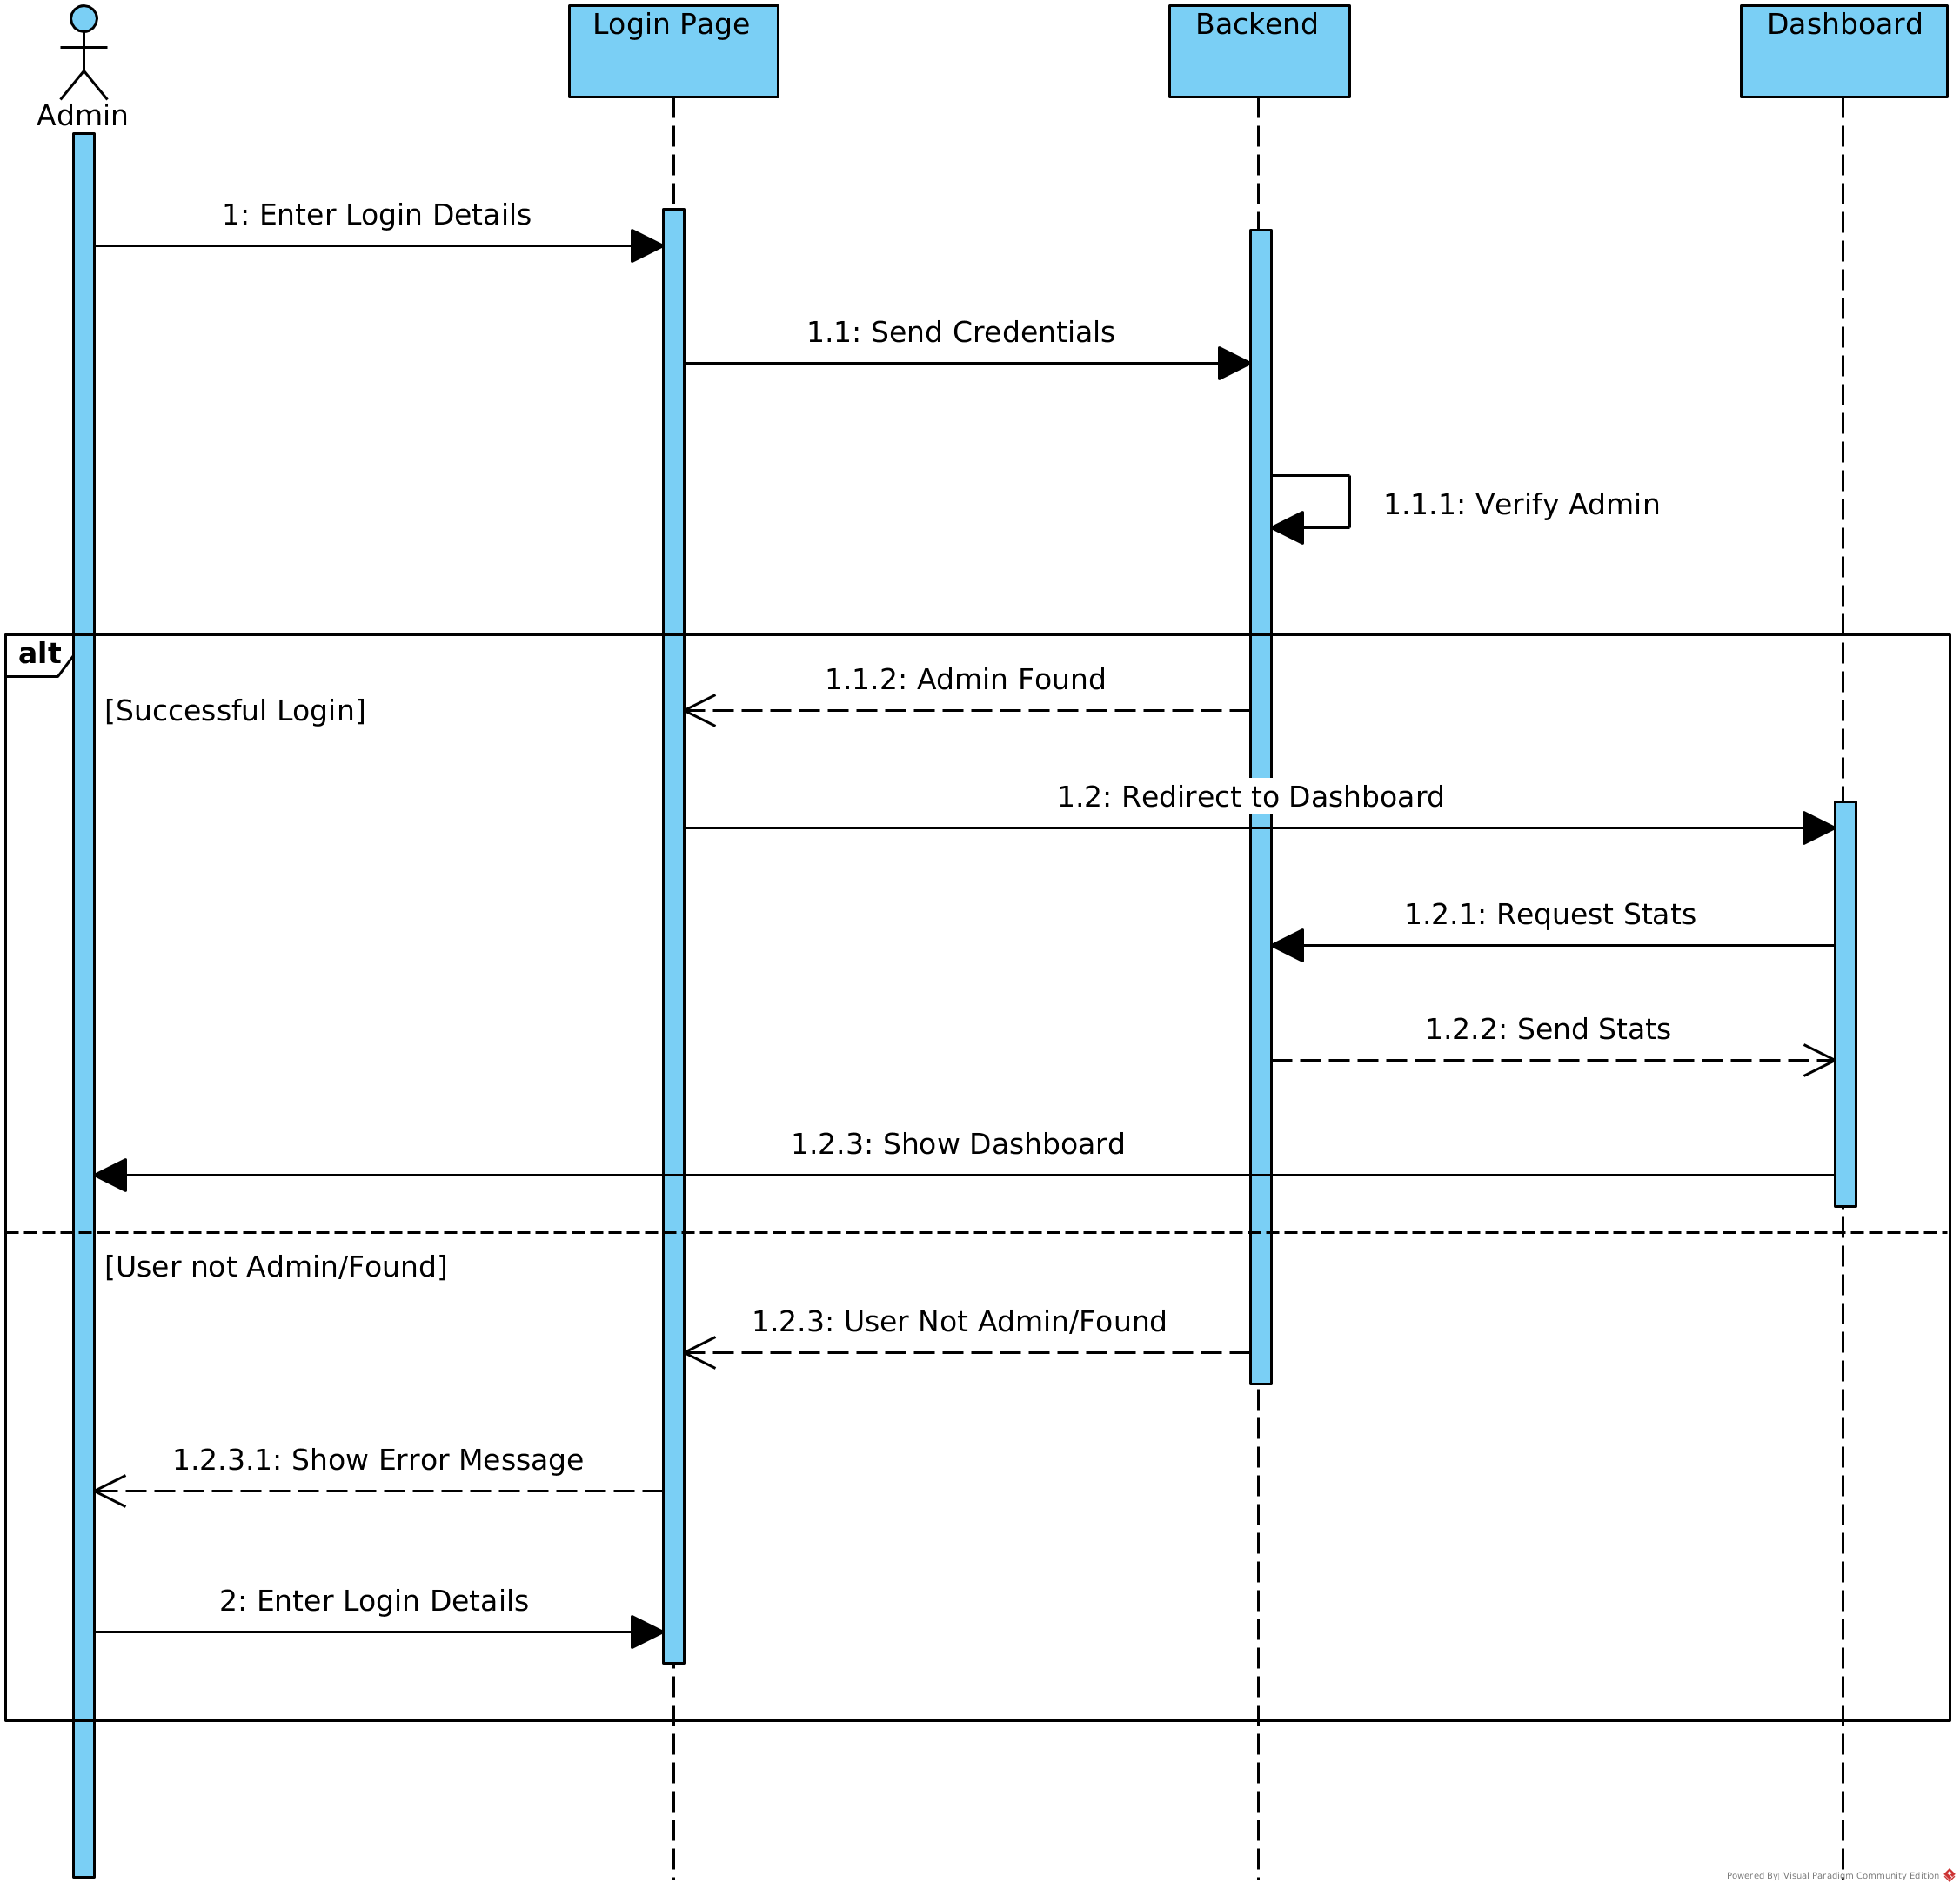
\includegraphics[width = \linewidth]{media/Sequence/Admin_Login.png}
	\caption{Admin Login: Sequence Diagram}
	\label{fig:Admin_Login}
\end{figure}


\begin{figure}[H]
    \centering
    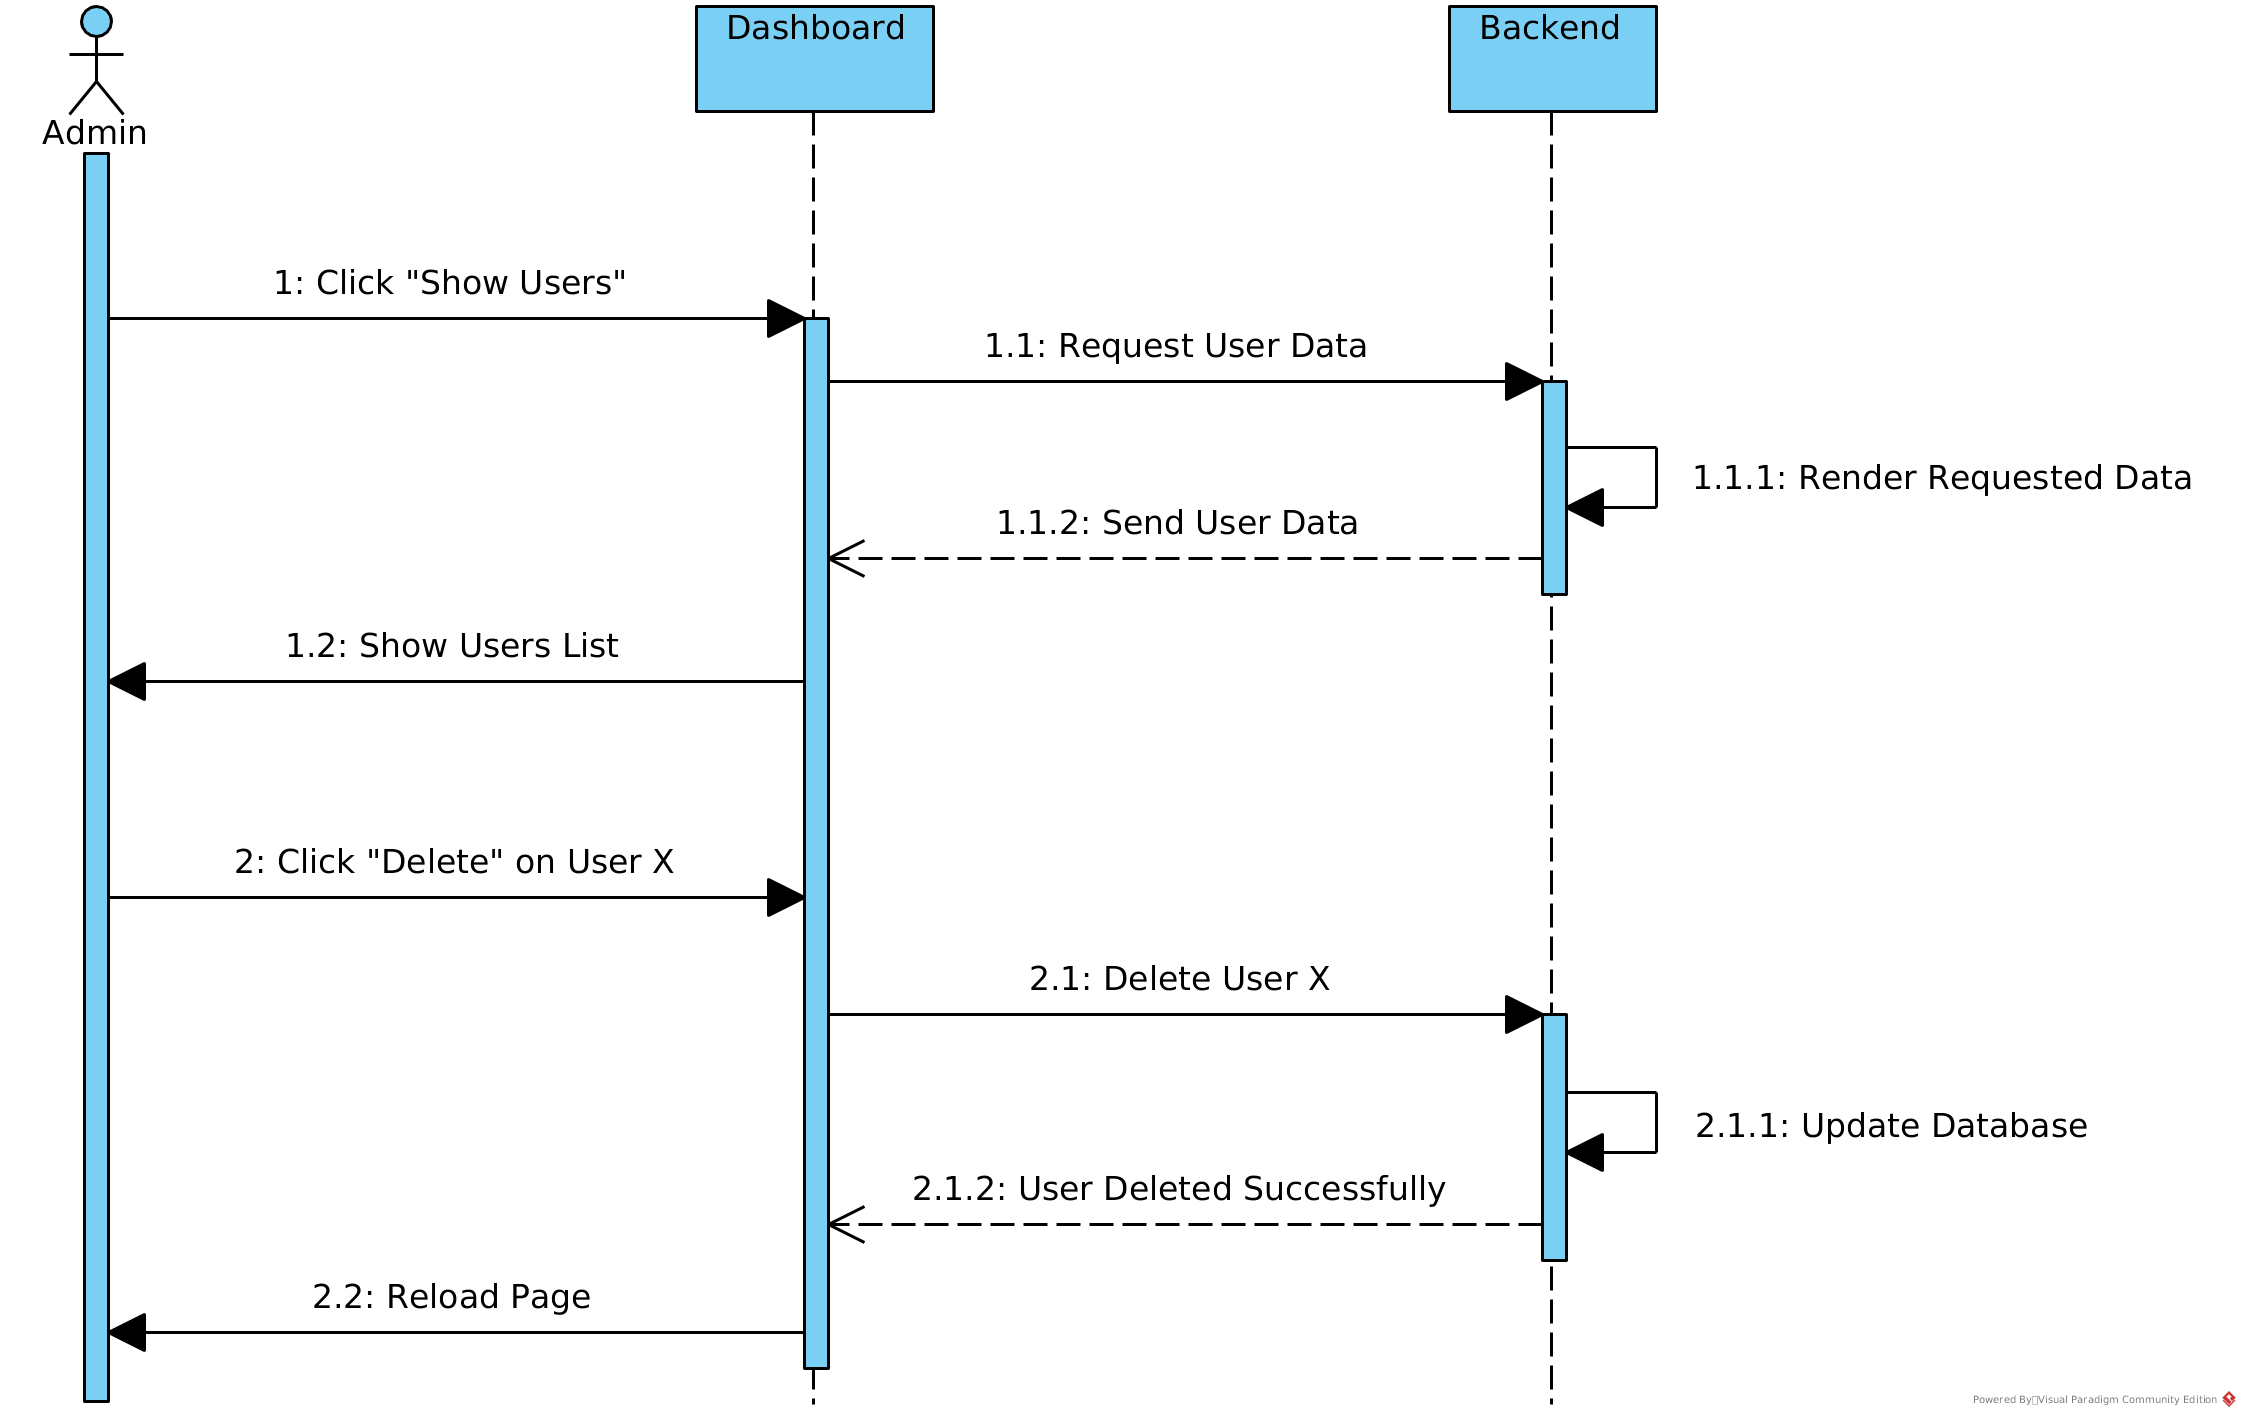
\includegraphics[width = \linewidth]{media/Sequence/Admin_Delete_User.png}
	\caption{Admin Delete User: Sequence Diagram}
	\label{fig:Admin_Delete_User}
\end{figure}

\begin{figure}[H]
    \centering
    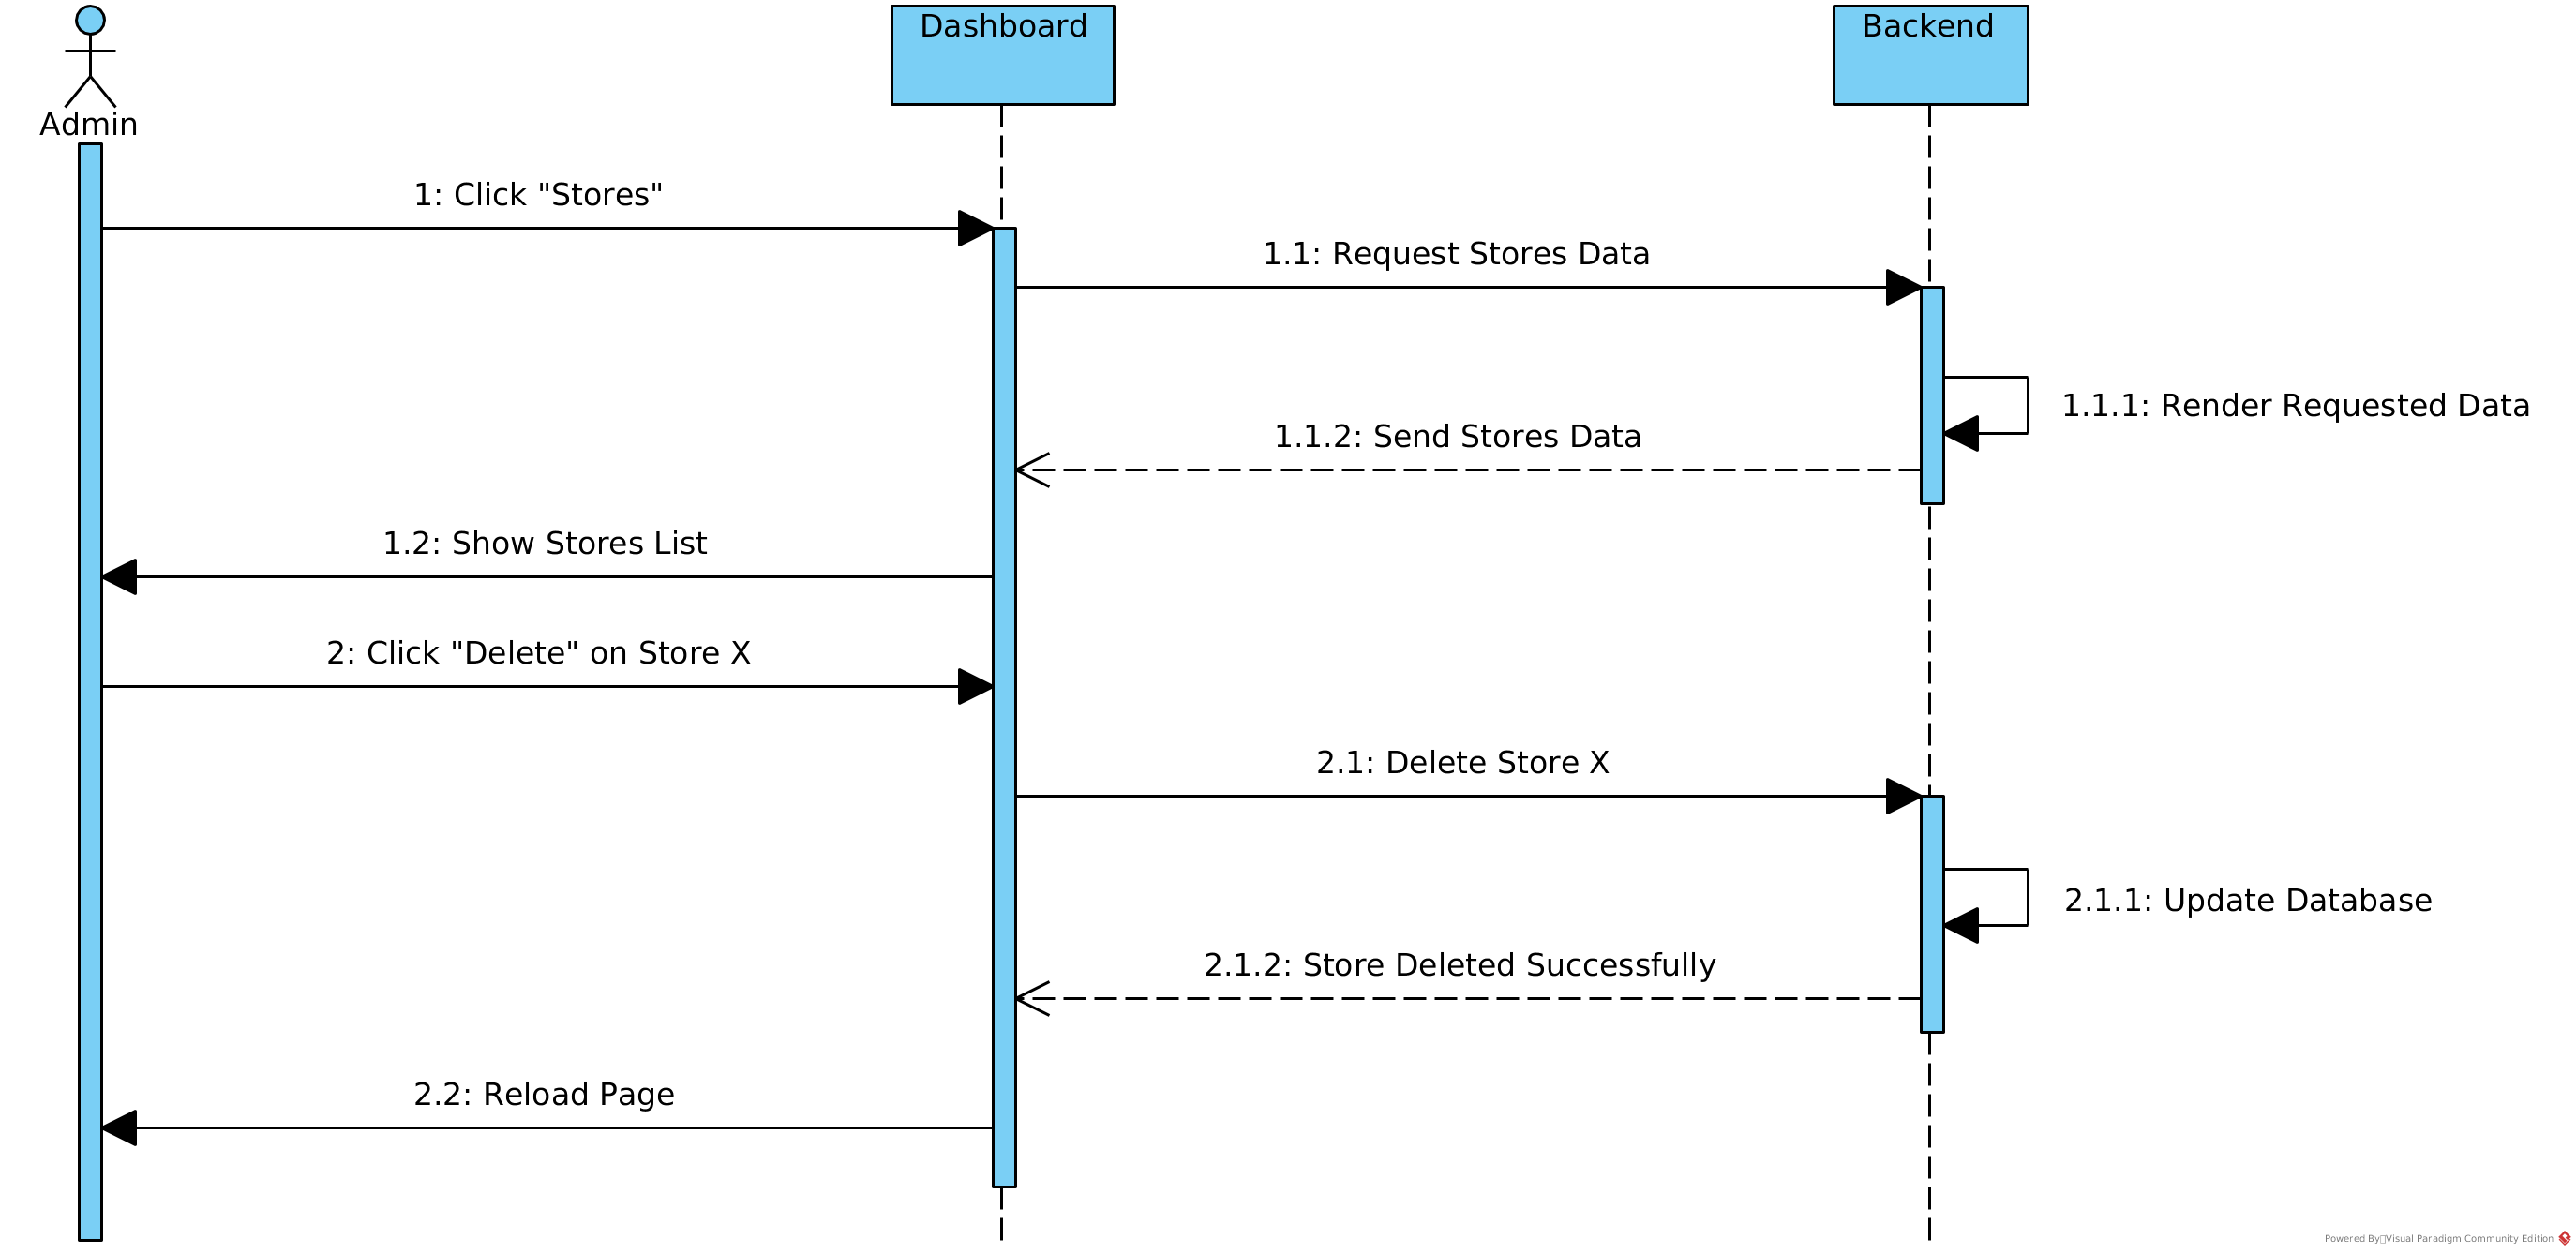
\includegraphics[width = \linewidth]{media/Sequence/Admin_Delete_Store.png}
	\caption{Admin Delete Store: Sequence Diagram}
	\label{fig:Admin_Delete_Store}
\end{figure}


\begin{figure}[H]
    \centering
    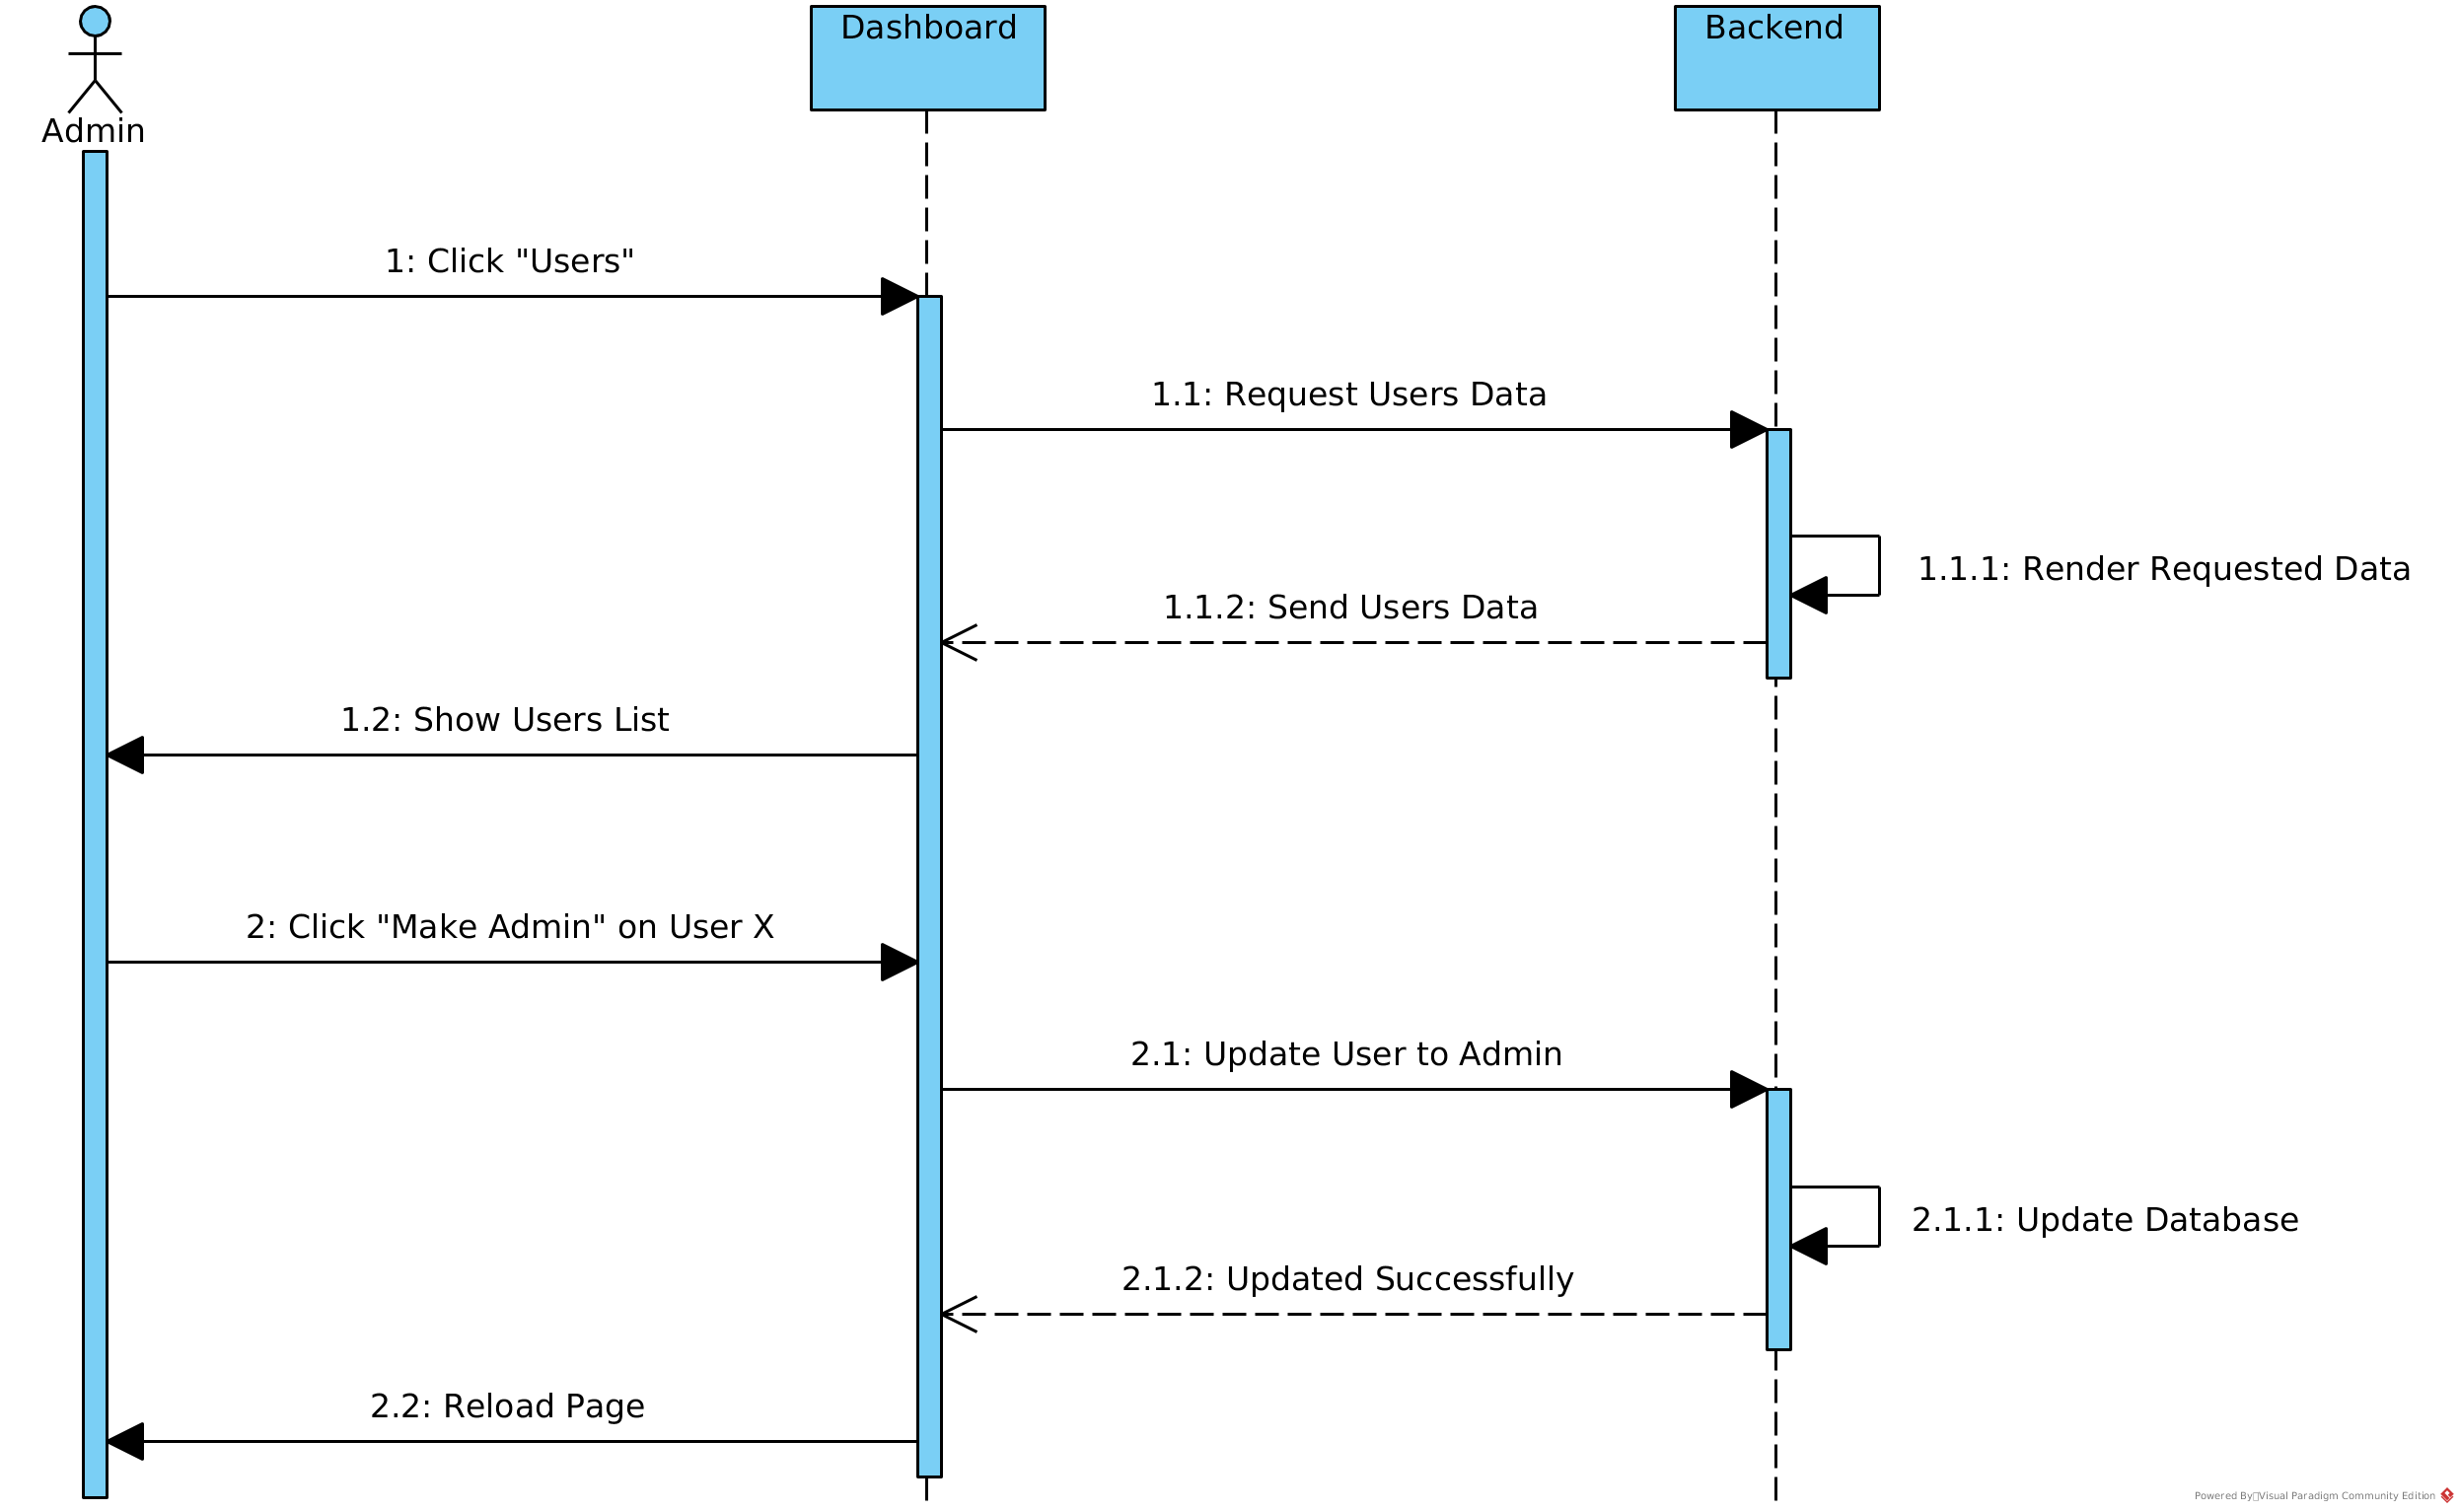
\includegraphics[width = \linewidth]{media/Sequence/Admin_Update_User.png}
	\caption{Admin Update User: Sequence Diagram}
	\label{fig:Admin_Update_User}
\end{figure}